\chapter{Problem Definition and Existing Solution}

\section{Problem Definition}
Given a natural-language task (for example, "book a one-way flight from Ahmedabad to Delhi on 12th May") and the current state of a live web page, the job of a web-automation agent is to produce the next executable step in a structured form. At each step the agent has to output a triple of (element, action, value), where the element is a concrete DOM node on the page, the action is one of the primitive interactions supported by the browser (click, type, select, and a few others), and the value is a string or null depending on the action. The page itself is observable in two representations, the rendered screenshot and the underlying HTML/DOM tree, and a real agent has to consume at least one of these at every step.

Three practical constraints turn this into a hard problem. First, modern pages routinely contain tens of thousands of DOM tokens \cite{zhang2025prune4web}, which is larger than the useful context window of most LLMs and expensive to send on every step. Second, the agent has to respect a per-step latency budget of a few seconds, otherwise the interaction does not feel live. Third, DOM elements in real websites carry user-sensitive values, such as email addresses, phone numbers, credit card fields, and identification numbers, so any sensible agent pipeline has to avoid leaking these values to a hosted LLM without the user's awareness. A useful web-automation system therefore has to reach high element-level accuracy while keeping token cost, latency, and privacy risk all within realistic limits.

In the third semester of this project, the base paper under study was SeeAct \cite{SeeAct}, which proposed a GPT-4V driven multimodal agent and introduced the Multimodal-Mind2Web dataset. SeeAct is still a useful reference for the motivation and the dataset, but it relies on GPT-4V at every step, which makes reproducing the full pipeline on a student setup infeasible from a billing point of view. For the Sem~IV work we therefore switched the anchor of our problem-definition chapter to a system that we could actually re-implement, run, and measure end-to-end on local hardware, namely Prune4Web.


\section{Existing Solution: Prune4Web}

Prune4Web (Zhang \textit{et al.}, 2025) \cite{zhang2025prune4web} is a three-stage pipeline for LLM-based web agents. It is the closest published system to the design we want and it explicitly targets the cost/context problem of sending the DOM to the LLM. Figure \ref{Prune4Web:Architecture} shows the high-level flow.

\begin{figure}[h]
    \centering
    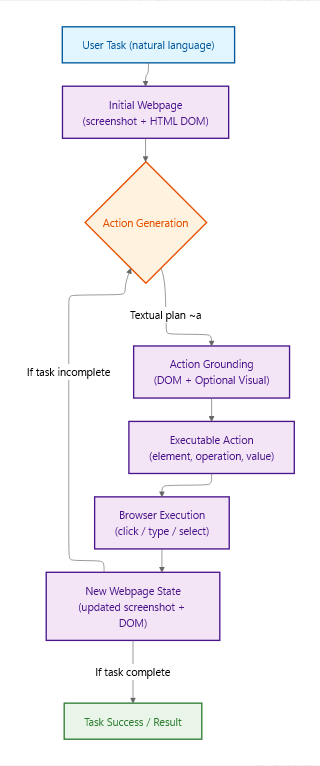
\includegraphics[width=0.75\linewidth]{SeeAct Diagram (white-BG).png}
    \caption{Prune4Web pipeline: Planner (LLM) $\to$ Programmatic Element Filter (LLM emits weights, Python scores) $\to$ Action Grounder (LLM on top-$N$ elements). Reproduced conceptually from \cite{zhang2025prune4web}; diagram to be replaced in the final version.}
    \label{Prune4Web:Architecture}
\end{figure}

    \subsection{Stage 1: Planner}
    A multimodal LLM receives the high-level task, the page screenshot, and the previous-step history, and emits a single JSON object with one \texttt{sub\_task} field (plus \texttt{action\_type}, \texttt{value}, and a short \texttt{reasoning} string). The planner breaks a long task like "buy a laptop under 50{,}000" into one imperative sub-task per step, for example "click the search box" \cite{zhang2025prune4web}. The planner never looks at the raw DOM.

    \subsection{Stage 2: Programmatic Element Filter}
    This is the core contribution of the paper. The LLM is asked to emit a small keyword/weight scoring script based only on the sub-task, without seeing any DOM content. A deterministic Python scorer then runs that script over every interactive DOM element, combining per-keyword weights with per-attribute importance (tag, visible text, id, name, aria-label, placeholder, title, role, class) and returns the top-$N$ candidates \cite{zhang2025prune4web}. Because the LLM never reads raw DOM at this stage, the filter call stays $O(\text{sub-task length})$ in tokens instead of $O(\text{page size})$, and the reported candidate reduction is 25x to 50x \cite{zhang2025prune4web}.

    \subsection{Stage 3: Action Grounder}
    A second LLM call receives the sub-task along with the compact block of top-$N$ element summaries and returns the exact target (\texttt{element\_uid}, \texttt{action}, \texttt{value}). On Mind2Web, Prune4Web reports 88.28\% Element Accuracy with a Qwen2.5VL-3B-Instruct vision-language grounder fine-tuned by the authors, and shows that a lighter Qwen2.5-0.5B-Instruct variant also operates in the same Filter-Grounder pipeline \cite{zhang2025prune4web}.

\noindent Overall, Prune4Web is a clean and measurable starting point because the filter and grounder stages are modular, the token-cost argument is verifiable, and the evaluation is on a standard benchmark (Mind2Web) that the earlier Sem-III work already used.


\section{Gaps We Inherit From Prune4Web}

Re-implementing Prune4Web in this repository and running it over the Mind2Web splits surfaced three gaps that directly motivate the proposed contributions in Chapter 4.

\textbf{Grounder leans on a 3B vision-language model.}
Prune4Web's headline 88.28\% Element Accuracy comes from a Qwen2.5VL-3B-Instruct grounder that the authors fine-tune themselves; a lighter Qwen2.5-0.5B-Instruct variant is also reported as a proof-of-concept but not as the primary result \cite{zhang2025prune4web}. Using a 3B vision-language grounder means the grounder always consumes the page screenshot in addition to the candidate element summaries, which pushes memory and latency well past what a 6~GB consumer GPU can serve, and the 0.5B text-only variant reported in the paper is not accompanied by LoRA hyperparameters, training schedule, or per-split accuracy that would let another group reproduce it. This leaves open whether a purely text-mode grounder below 1B parameters, trained with a documented recipe, can match the 3B VLM at element accuracy. Our QLoRA-tuned Qwen2.5-0.5B and Qwen3-0.6B grounders (Chapter 4 and 5) answer exactly that question.

\textbf{DOM processing is single-step and stateless.}
Each step of Prune4Web re-runs the filter on the full current DOM, even if the page has barely changed from the previous step. This is a wasted efficiency signal: in typical multi-step tasks a button click only opens a new dropdown, or fills in one field, yet the next step still ships the entire DOM back through the filter. Prune4Web, Mind2Web, AutoWebGLM, and D2Snap all share this limitation \cite{zhang2025prune4web} \cite{deng2023mind2webgeneralistagentweb} \cite{lai2024autowebglm} \cite{schiepanski2025d2snap}, and it is the gap that our DOM Delta Processing is designed to close.

\textbf{No privacy / HITL layer inside the loop.}
Prune4Web sends the candidate element summaries, which frequently contain PII in attributes like \texttt{value}, \texttt{placeholder}, and \texttt{aria-label}, straight to the grounder LLM without masking. It also has no notion of an action being risky on its own terms (payment, credential, CAPTCHA, destructive confirmations) and therefore no gate that can pause or escalate before the action is executed. Both safety and privacy concerns are flagged as open problems in recent surveys \cite{tang2025surveymllmbasedguiagents} \cite{ning2025surveywebagentsnextgenerationai}, and the Privacy Hub + HITL layer in Chapter 4 is our response to this gap.

\bigskip
\noindent These three gaps (local grounder, cross-step DOM reduction, privacy-aware execution) are the direct motivation for the proposed methodology described in Chapter 4 and evaluated in Chapter 5.
